\documentclass{article}

\usepackage[a4paper,top=2cm,bottom=2cm,left=3cm,right=3cm,marginparwidth=1.75cm]{geometry}
\usepackage[ngerman]{babel}
\usepackage{graphicx}
\usepackage{hyperref}
\usepackage{float}

\title{ERA Übungsaufgaben W22/23}
\author{David Erb}
\begin{document}
\maketitle

\section{Einführung}
Dieses Aufgabenblatt wurde von Studenten erstellt, um zusätzliche Aufgaben für die Klausurvorbereitung bereitzustellen. Somit kann nicht für die Relevanz der Aufgaben im Bezug auf die Klausur bzw. für korrekte Lösungsvorschläge garantiert werden.

\section{Aufgaben}

\subsection{Aufgabe 1}
Einige Pinguine an der PUM sind Workaholics und machen viele, Fehler wenn sie zu lange am Stück arbeiten. Daher hat ein Pinguin eine Ampelschaltung  entworfen, welche den Workaholics anzeigen soll, wann sie eine Pause machen sollen. Die Schaltung hat 4 Zustände: Grün(Startzustand), Gelb, Rot und Pause. Jedes Mal wenn ein Pinguin einen Fehler(Input = 1) macht, soll sich der Zustand der Ampel um eins verschlechtern. Von Rot gerät man dabei in den Pause-Zustand, den man bei keiner der Input-Werte verlässt. Macht der Pinguin bei einer Aufgabe keinen Fehler(Input = 0), während die Schaltung nicht im Pause-Zustand ist, schaltet die Ampel wieder auf grün. Die Ampel ist also im Pause-Zustand wenn der Pinguin irgendwann einmal drei Fehler in Folge gemacht hat. Nur in dem Pause-Zustand soll die Ampel dem Pinguin das Signal geben, eine Pause zu machen (Output = 1)
(\hyperref[sec:lsg01]{Lösungsvorschlag}). \\
\\
i) Zeichne den Moore-Automat dieser Schaltung.\\
\\
ii) Fülle die Wahrheitstabelle der Zustandsübergangsfunktion des Automaten aus. Die Zustände haben folgende Binärkodierung: \\
Grün: 00 \\
Gelb: 01 \\
Rot: 10 \\
Pause 11 \\
\texttt{FFn} ist dabei das \texttt{n}te Bit des Zustands und \texttt{FFn'} das jeweilige Bit des Folgezustands.\\
I ist der Input, O der Output.\\ 
\\
\begin{tabular}{c|c|c|c|c|c|c}
   I  & FF1 & FF0 & FF1' & FF0' & O \\
    \hline
   0   &  0   & 0   &      &      &   \\
    \hline
   0  &   0  &  1   &      &      &   \\
     \hline
   0  &  1   &  0   &      &      &   \\
     \hline
   0  &   1  &  1   &      &      &   \\
     \hline
   1  &  0   &  0   &      &      &   \\
     \hline
   1  &   0  &  1   &      &      &   \\
     \hline
   1  &  1   &  0   &      &      &   \\
     \hline
   1  &  1   &   1  &      &      &   \\
     \hline
\end{tabular} \\
\\
iii) Gib den boolschen Term von \texttt{FF0'} an.

\newpage

\section{Lösungsvorschläge}

\subsection{Aufgabe 1 (Lösungsvorschlag)} \\
i)
\begin{figure}[H]
\centering
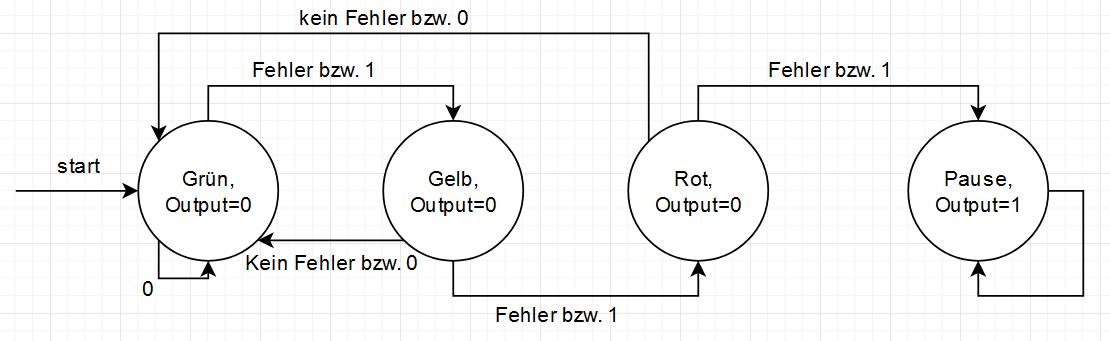
\includegraphics[scale=0.45]{automat.png}
\caption{Moore-Automat der Ampelschaltung}
\end{figure}

ii) \\
\\
\begin{tabular}{c|c|c|c|c|c|c}
   I  & FF1 & FF0 & FF1' & FF0' & O \\
    \hline
   0   &  0   & 0   &   0   &   0   & 0  \\
    \hline
   0  &   0  &  1   &  0    &   0   &  0 \\
     \hline
   0  &  1   &  0   &   0   &   0   & 0  \\
     \hline
   0  &   1  &  1   &   1   &   1   & 1  \\
     \hline
   1  &  0   &  0   &   0   &   1   &  0 \\
     \hline
   1  &   0  &  1   &   1   &   0   &  0 \\
     \hline
   1  &  1   &  0   &   1   &   1   & 0  \\
     \hline
   1  &  1   &   1  &   1   &   1   &  1 \\
     \hline
\end{tabular} \\
 \\
iii) \\
\\
\texttt{FF0' = FF1 FF0 + I $\neg FF0$}
\label{sec:lsg01}

\end{document}
